\section*{Experiments}

We quantitatively compare our method against previous works for multi-view shape generation in~\tableref{baseline_comparison_cd} and show effectiveness of our proposed shape generation methods in improving shape quality. Our method outperforms the state-of-the-art method  Pixel2Mesh++~\cite{wen2019pixel2mesh++} with
decrease in chamfer distance to ground truth by 34\%, which shows the effectiveness of our proposed method.
Note that in~\tableref{baseline_comparison_cd} same model is trained for all the categories but accuracy on individual categories as well as average over all the categories are evaluated.

\begin{table}[ht]
\begin{center}
% \resizebox{\linewidth}{!}{
\begin{tabular}{|c|ccccc|}
    \hline
    \multirow{2}{*}{Category}&
    \multicolumn{5}{c|}{Chamfer Distance (CD) $\downarrow$} \\
    & 3D-R2N2 & LSM & MVP2M & P2M++ & \bf{Ours} \\
    \hline
    Couch       & 0.806 & 0.730 & 0.534 & 0.439 & \bf{0.220} \\
    Cabinet     & 0.613 & 0.634 & 0.488 & 0.337 & \bf{0.230} \\
    Bench       & 1.362 & 0.572 & 0.591 & 0.549 & \bf{0.159} \\
    Chair       & 1.534 & 0.495 & 0.583 & 0.461 & \bf{0.201} \\
    Monitor     & 1.465 & 0.592 & 0.658 & 0.566 & \bf{0.217} \\
    Firearm     & 0.432 & 0.385 & 0.305 & 0.305 & \bf{0.123} \\
    Speaker     & 1.443 & 0.767 & 0.745 & 0.635 & \bf{0.402} \\
    Lamp        & 6.780 & 1.768 & 0.980 & 1.135 & \bf{0.755} \\
    Cellphone   & 1.161 & 0.362 & 0.445 & 0.325 & \bf{0.138} \\
    Plane       & 0.854 & 0.496 & 0.403 & 0.422 & \bf{0.084} \\
    Table       & 1.243 & 0.994 & 0.511 & 0.388 & \bf{0.181} \\
    Car         & 0.358 & 0.326 & 0.321 & 0.249 & \bf{0.165} \\
    Watercraft  & 0.869 & 0.509 & 0.463 & 0.508 & \bf{0.175} \\
    \hline
    Mean        & 1.455 & 0.664 & 0.541 & 0.486 & \bf{0.211} \\
    \hline
\end{tabular}
% }
\end{center}
\caption{
    \textbf{Qualitative comparison} against state-of-the-art multi-view shape generation methods. Following~\cite{wen2019pixel2mesh++}, we report Chamfer Distance in $m^2 \times 1000$ from ground truth for different methods. Note that same model is trained for all the categories but accuracy on individual categories as well as average over all the categories are evaluated.
}
\label{table:baseline_comparison_cd}
\end{table}



\subsection*{Ablation studies}

\vspace{-2mm}
\paragraph{Coarse Shape Generation}
We conduct comparisons on voxel grid predicted from our proposed probabilistically merged voxel grids against single view method~\cite{gkioxari2019meshrcnn}.
As is shown in~\tableref{multiview_voxel_accuracy}, the accuracy of the initial shape generated from probabilistically merged voxel grid is higher than that from individual views.
% \tableref{multiview_voxel_accuracy} also evaluates different input modalities for voxel prediction among which RGB image concataneted with depth image produces best results.
% Note that the \emph{voxel branch} (~\subsecref{multiview_voxel}) was trained and tested separately for each of the cases without mesh refinement.

% \begin{table}[ht]
% \begin{center}
% \footnotesize
% \begin{tabular}{c | c c c c c c}
%     \hline
%     Metric & RGB-Ours & Depth-Ours & RGBD-Ours & RGB 1-view & Depth 1-view & RGBD 1-view \\
%     \hline
%     F1-$\tau$   & 31.27 & 30.30 & 31.61 & 25.19 & 23.78 & 26.06 \\
%     F1-$2\tau$  & 44.46 & 43.16 & 44.86 & 36.75 & 35.14 & 37.74 \\
%     \hline
% \end{tabular}
% \end{center}
% \caption{
%     Accuracy of predicted voxel of individual views against probabilistically merged multi-view voxel grids, where the first three columns indicate the accuracy of multi-view voxel generations while the last three columns show single-view. The voxel branch was trained separately without the mesh refinement. Evaluation is conducted after cubify and the depth maps are generated from MVSNet.
% }
% \label{table:multiview_voxel_accuracy}
% \end{table}
\begin{table}[ht]
\noindent \scriptsize \footnotesize
\begin{minipage}[t]{0.5\textwidth}
\centering
\begin{tabular}{c | c c}
    \hline
    Metric      & Single-view & Multi-view \\
    \hline
    F1-$\tau$   & 25.19 & 31.27 \\
    F1-$2\tau$  & 36.75 & 44.46 \\
    \hline
\end{tabular}
\caption{
    \textbf{Accuracy of predicted voxel grids} from single-view prediction compared against the proposed probabilistically merged multi-view voxel grids. The voxel branch was trained separately without the mesh refinement and evaluation was performed on the cubified voxel grids. We use three views for probabilistic grid merging.
}
\label{table:multiview_voxel_accuracy}
\end{minipage}
\hspace{0.1cm}
\noindent \scriptsize \footnotesize
\begin{minipage}[t]{0.5\textwidth}
\centering
\begin{tabular}{c | c c c c}
    \hline
    Metric & Cubified & Stage-1 & Stage-2 & Stage-3 \\
    \hline
    F1-$\tau$   & 31.48 & 76.78 & 79.88 & 80.80  \\
    F1-$2\tau$  & 44.40 & 88.32 & 90.19 & 90.72  \\
    \hline
\end{tabular}
\caption{
    \textbf{Accuracy of the refined meshes at different GCN stages}. 1, 2 and 3 indicate the performance at the corresponding graph convolution blocks while \emph{Cubified} is for the cubified voxel grids used as input for the first GCN block. All the stages, including the voxel prediction, were trained jointly and hence the accuracy of voxel predictions varies from that in~\tableref{multiview_voxel_accuracy}.
}
\label{table:gcn_stages}
\end{minipage}
\end{table}


\vspace{-2mm}
\paragraph{Resolution of Depth Prediction}
We conduct experiments using different numbers of depth hypotheses in our depth prediction network (\subsecref{mvsnet}), producing depth values at different resolutions.
A higher number of depth hypothesis means finer resolution of the predicted depths.
The quantitative results with different hypothesis numbers are summarized in~\tableref{depth_resolution}. We set depth hypothesis as $48$ for our final architecture which is equivalent to the resolution of $25$ mm.
We observe that the mesh accuracy remain relatively unchanged if we predict depths at finer resolutions.
% We evaluate the performance at different number of depth hypothesis of the depth prediction model (\subsecref{depth_prediction} ).
% As can be seen in~\tableref{depth_resolution}, the performance of the model with different number of depth hypotheses are roughly the same. Note that the range of depth values for all the models are kept the same.
\begin{table}[ht]
% \captionsetup{font=footnotesize,labelfont=footnotesize}
\begin{center}
\footnotesize
\begin{tabular}{l | c c c c}
    \hline
    Metric & 24 & 48 & 72 & 96  \\
    \hline
    F1-$\tau$  & 80.29 & 80.80 & 80.69 & 80.34   \\
    F1-$2\tau$ & 90.43 & 90.72 & 90.74 & 90.47   \\
    \hline
\end{tabular}
\end{center}
\caption{
    \textbf{Accuracy w.r.t the number of depth hypothesis}. A higher number of depth hypothesis increases the resolution of predicted depth values at the expense of higher memory requirement. The range of depths for all the models are same and based on the minimum/maximum depth in the ShapeNet~\cite{chang2015shapenet} dataset.
}
\label{table:depth_resolution}
\end{table}


\paragraph{Attention Weights visualization}
We visualize the learned attention weights (average of each attention heads) in~\figref{attention_weights} where we can observe that the attention weights roughly takes into account the visibility/occlusion information from each view.
\begin{figure*}[t]
\begin{center}
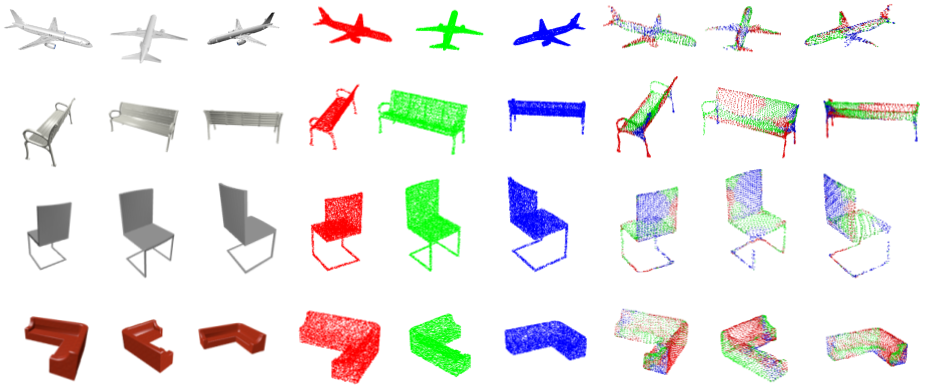
\includegraphics[width=\linewidth]{imgs/attention_weights_visualization.png}
\end{center}
    \caption{
        \textbf{Attention weights visualization.}
        From left to right: input images from 3 viewpoints, corresponding ground truth point clouds color-coded by their view order and the predicted mesh vertices color-coded by the attention weights of the views.
        Only the view with maximum attention weight is visualized for each predicted points for clarity.
    }
\label{fig:attention_weights}
\end{figure*}

